\newcommand{\dropperTagResultsAucTable}{
    \begin{table}[H]
        \centering
        \begin{tabular}{|p{2,8cm}||P{2,2cm} P{2,2cm} P{2,2cm} P{2,2cm}|}
            \hline
            Dropper Tag & ALOHA\newline (M/B only) & ALOHA & Joint\newline Embedding & Proposed\newline Model \\
            \hline
            AUC-ROC & - & 0.968$\pm$0.005 & 0.972$\pm$0.001 & \textBF{0.977$\pm$0.001} \\
            \hline
        \end{tabular}
        \caption[Dropper Tag prediction task AUC-ROC results]{AUC-ROC (Area Under Curve) of the different models for the \textbf{Dropper Tag} prediction task. Results were aggregated over \textBF{3} training runs with different weight initializations and minibatch orderings. Best results are shown in \textbf{bold}.} \label{tab:dropperTag_auc}
    \end{table}
}

\newcommand{\dropperTagResultsAtFprTable}{
    \begin{center}
        \begin{longtable}[c]{|P{3,2cm}||P{1,8cm} P{1,8cm} P{1,8cm} P{1,8cm} P{1,8cm}|}
            \hline
            Dropper Tag & \multicolumn{5}{c|}{{FPR}} \\
            & $10^{-5}$ & $10^{-4}$ & $10^{-3}$ & $10^{-2}$ & $10^{-1}$ \\
            \hline
            \endfirsthead

            \caption*{\raggedright ...continued from previous page} \\
            \hline
            Dropper Tag & \multicolumn{5}{c|}{\textbf{FPR}} \\
            & $10^{-5}$ & $10^{-4}$ & $10^{-3}$ & $10^{-2}$ & $10^{-1}$ \\
            \hline
            \endhead

            \caption*{\raggedleft ...continued on next page} \\
            \endfoot

            \caption[Dropper Tag prediction task results]{Mean and standard deviation results (TPR, Accuracy, Recall, Precision and F1-Score) of the different models for the \textbf{Dropper Tag} prediction task at different \textbf{FPR}s (\textit{False Positive Rates}). Results were aggregated over \textBF{3} training runs with different weight initializations and minibatch orderings. Best results are shown in \textbf{bold}. Under \textbf{TPR} results are also presented the percentage reduction in mean detection error and in ROC curve standard deviation introduced by the \textit{Proposed Model} with respect to both \textit{ALOHA} model and \textit{Joint Embedding}.} \label{tab:dropperTag_results_at_fpr} \\
            \endlastfoot

            \multicolumn{6}{|c|}{\textbf{TPR}} \\
            \hline
            ALOHA (M/B only) & - & - & - & - & - \\
            ALOHA & 0.042$\pm$0.022 & 0.073$\pm$0.023 & 0.127$\pm$0.053 & 0.673$\pm$0.037 & 0.899$\pm$0.017 \\
            Joint Embedding & \textBF{0.088$\pm$0.088} & 0.104$\pm$0.089 & \textBF{0.176$\pm$0.130} & \textBF{0.702$\pm$0.031} & 0.904$\pm$0.019 \\
            Proposed Model & 0.068$\pm$0.015 & \textBF{0.127$\pm$0.047} & 0.151$\pm$0.042 & 0.690$\pm$0.016 & \textBF{0.943$\pm$0.017} \\
            \hline
            Error Reduction wrt\newline ALOHA (M/B only) & - & - & - & - & - \\
            Error Reduction wrt\newline ALOHA & 2.7\% & 5.8\% & 2.7\% & 5.2\% & 43.6\% \\
            Error Reduction wrt\newline Joint Embedding & -2.2\% & 2.6\% & -3.0\% & -4.0\% & 40.6\% \\
            \hline
            Std Reduction wrt\newline ALOHA (M/B only) & - & - & - & - & - \\
            Std Reduction wrt\newline ALOHA & 31.8\% & -104.3\% & 20.8\% & 56.8\% & 0.0\% \\
            Std Reduction wrt\newline Joint Embedding & 83.0\% & 47.2\% & 67.7\% & 48.4\% & 10.5\% \\
            \hline
            \multicolumn{6}{|c|}{\textbf{Accuracy}} \\
            \hline
            ALOHA (M/B only) & - & - & - & - & - \\
            ALOHA & 0.878$\pm$0.003 & 0.882$\pm$0.003 & 0.888$\pm$0.007 & 0.950$\pm$0.005 & 0.900$\pm$0.002 \\
            Joint Embedding & \textBF{0.884$\pm$0.011} & 0.886$\pm$0.011 & \textBF{0.894$\pm$0.016} & \textBF{0.953$\pm$0.004} & 0.901$\pm$0.002 \\
            Proposed Model & 0.881$\pm$0.002 & \textBF{0.888$\pm$0.006} & 0.891$\pm$0.005 & 0.952$\pm$0.002 & \textBF{0.905$\pm$0.002} \\
            \hline
            \multicolumn{6}{|c|}{\textbf{Recall}} \\
            \hline
            ALOHA (M/B only) & - & - & - & - & - \\
            ALOHA & 0.042$\pm$0.022 & 0.073$\pm$0.023 & 0.127$\pm$0.054 & 0.673$\pm$0.037 & 0.899$\pm$0.017 \\
            Joint Embedding & \textBF{0.088$\pm$0.088} & 0.104$\pm$0.089 & \textBF{0.174$\pm$0.129} & \textBF{0.702$\pm$0.031} & 0.904$\pm$0.019 \\
            Proposed Model & 0.066$\pm$0.014 & \textBF{0.126$\pm$0.047} & 0.150$\pm$0.042 & 0.690$\pm$0.016 & \textBF{0.943$\pm$0.017} \\
            \hline
            \multicolumn{6}{|c|}{\textbf{Precision}} \\
            \hline
            ALOHA (M/B only) & - & - & - & - & - \\
            ALOHA & 0.998$\pm$0.001 & 0.989$\pm$0.004 & 0.937$\pm$0.031 & 0.908$\pm$0.005 & 0.568$\pm$0.005 \\
            Joint Embedding & 0.991$\pm$0.012 & 0.946$\pm$0.069 & 0.880$\pm$0.130 & \textBF{0.911$\pm$0.004} & 0.570$\pm$0.005 \\
            Proposed Model & \textBF{0.999$\pm$0.000} & \textBF{0.994$\pm$0.002} & \textBF{0.954$\pm$0.011} & 0.910$\pm$0.002 & \textBF{0.580$\pm$0.004} \\
            \hline
            \multicolumn{6}{|c|}{\textbf{F1 Score}} \\
            \hline
            ALOHA (M/B only) & - & - & - & - & - \\
            ALOHA & 0.080$\pm$0.041 & 0.134$\pm$0.041 & 0.220$\pm$0.085 & 0.772$\pm$0.026 & 0.696$\pm$0.009 \\
            Joint Embedding & \textBF{0.149$\pm$0.144} & 0.176$\pm$0.146 & \textBF{0.274$\pm$0.191} & \textBF{0.793$\pm$0.021} & 0.699$\pm$0.009 \\
            Proposed Model & 0.124$\pm$0.026 & \textBF{0.221$\pm$0.072} & 0.258$\pm$0.062 & 0.785$\pm$0.011 & \textBF{0.718$\pm$0.008} \\
            \hline
        \end{longtable}
    \end{center}
}

\newcommand{\dropperTagResultsSummaryTable}{
    \begin{table}[H]
        \centering
        \begin{tabular}{|P{3,2cm}||P{1,8cm} P{1,8cm} P{1,8cm} P{1,8cm} P{1,8cm}|}
            \hline
            \multicolumn{6}{|c|}{Dropper Tag (at FPR $=1\%$)} \\
            \hline
            Model & TPR & Accuracy & Precision & Recall & F1 score \\
            \hline
            ALOHA (M/B only) & - & - & - & - & - \\
            ALOHA & 0.673$\pm$0.037 & 0.950$\pm$0.005 & 0.908$\pm$0.005 & 0.673$\pm$0.037 & 0.772$\pm$0.026 \\
            Joint Embedding & \textBF{0.702$\pm$0.031} & \textBF{0.953$\pm$0.004} & \textBF{0.911$\pm$0.004} & \textBF{0.702$\pm$0.031} & \textBF{0.793$\pm$0.021} \\
            Proposed Model & 0.690$\pm$0.016 & 0.952$\pm$0.002 & 0.910$\pm$0.002 & 0.690$\pm$0.016 & 0.785$\pm$0.011 \\
            \hline
        \end{tabular}
        \caption[Summary of Dropper Tag prediction task results]{Summary of the mean and standard deviation results of the different models for the \textbf{Dropper Tag} prediction task at \textbf{FPR} $=1\%$. Results were aggregated over \textBF{3} training runs with different weight initializations and minibatch orderings. Best results are shown in \textbf{bold}.} \label{tab:dropperTag_result_summary}
    \end{table}
}

\newcommand{\dropperTagRocAlohaMB}{
    \begin{figure}[H]
        \vspace*{-0.5cm}
        \centering
        \includegraphics[width=0.6\textwidth]{./results/dropper_tag_roc_alohaMB.png}
        \vspace*{-0.2cm}
        \caption[Dropper Tag prediction task ALOHA (M/B only) ROC curve]{ROC curve and AUC statistics of \textBF{ALOHA (M/B only)} model for the \textbf{Dropper Tag}. The line represents the \textit{mean} TPR at a given FPR, while the shaded region represents the \textit{standard deviation}. Statistics were computed over \textBF{3} training runs, each with random parameter initialization.}
        \label{fig:dropperTagRocAlohaMB}
    \end{figure}
}

\newcommand{\dropperTagRocAloha}{
    \begin{figure}[H]
        \vspace*{-0.5cm}
        \centering
        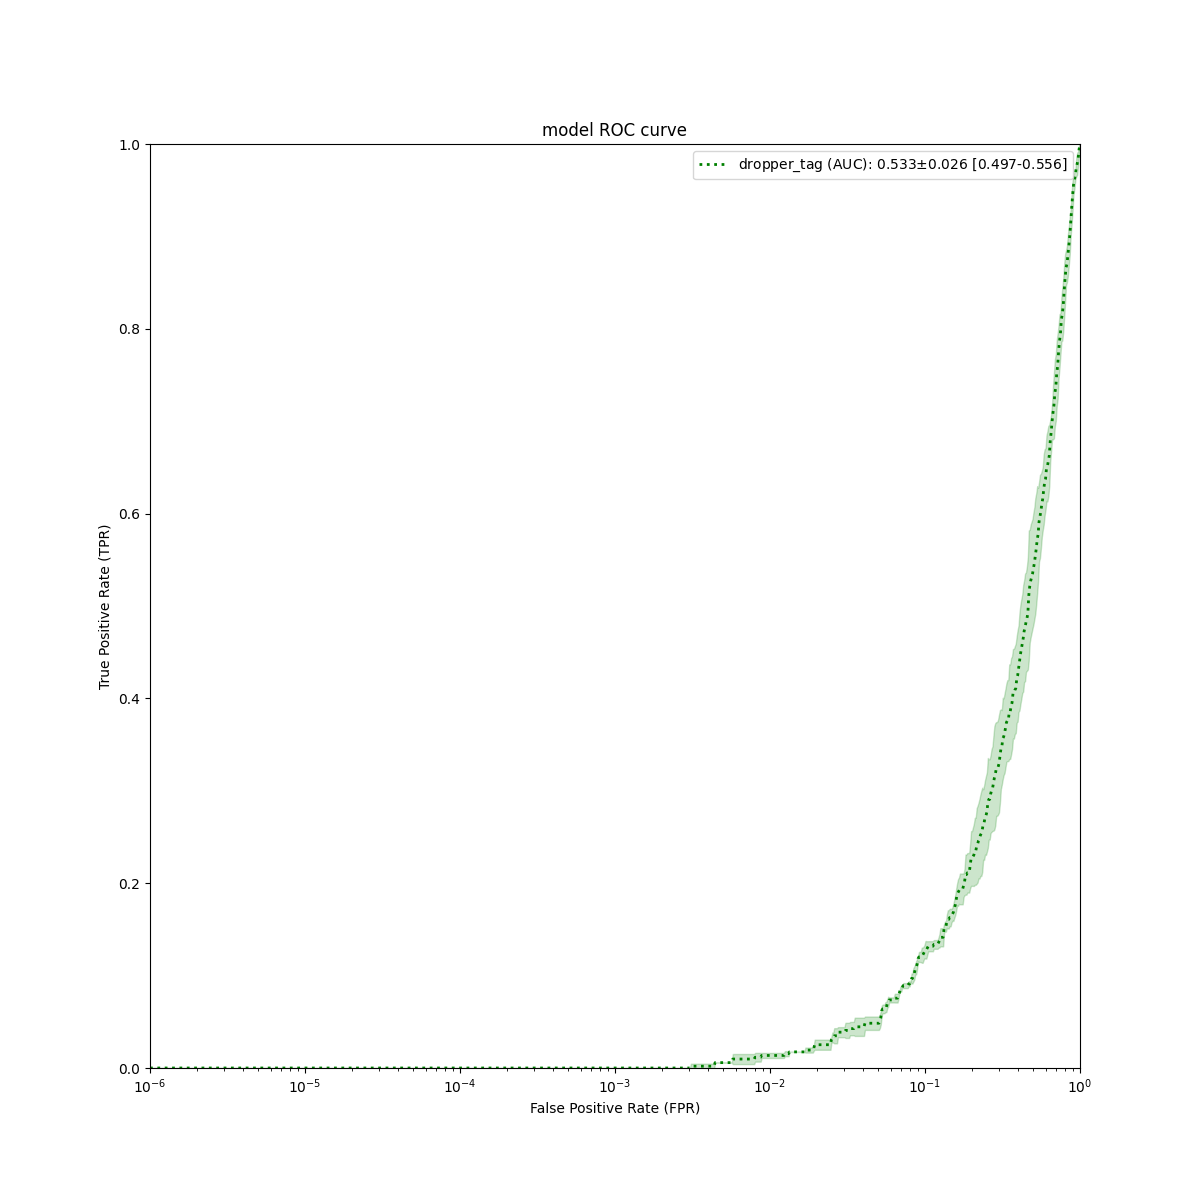
\includegraphics[width=0.6\textwidth]{./results/dropper_tag_roc_aloha.png}
        \vspace*{-0.2cm}
        \caption[Dropper Tag prediction task ALOHA ROC curve]{ROC curve and AUC statistics of \textBF{ALOHA} model for the \textbf{Dropper Tag}. The line represents the \textit{mean} TPR at a given FPR, while the shaded region represents the \textit{standard deviation}. Statistics were computed over \textBF{3} training runs, each with random parameter initialization.}
        \label{fig:dropperTagRocAloha}
    \end{figure}
}

\newcommand{\dropperTagRocJointEmbedding}{
    \begin{figure}[H]
        \vspace*{-0.5cm}
        \centering
        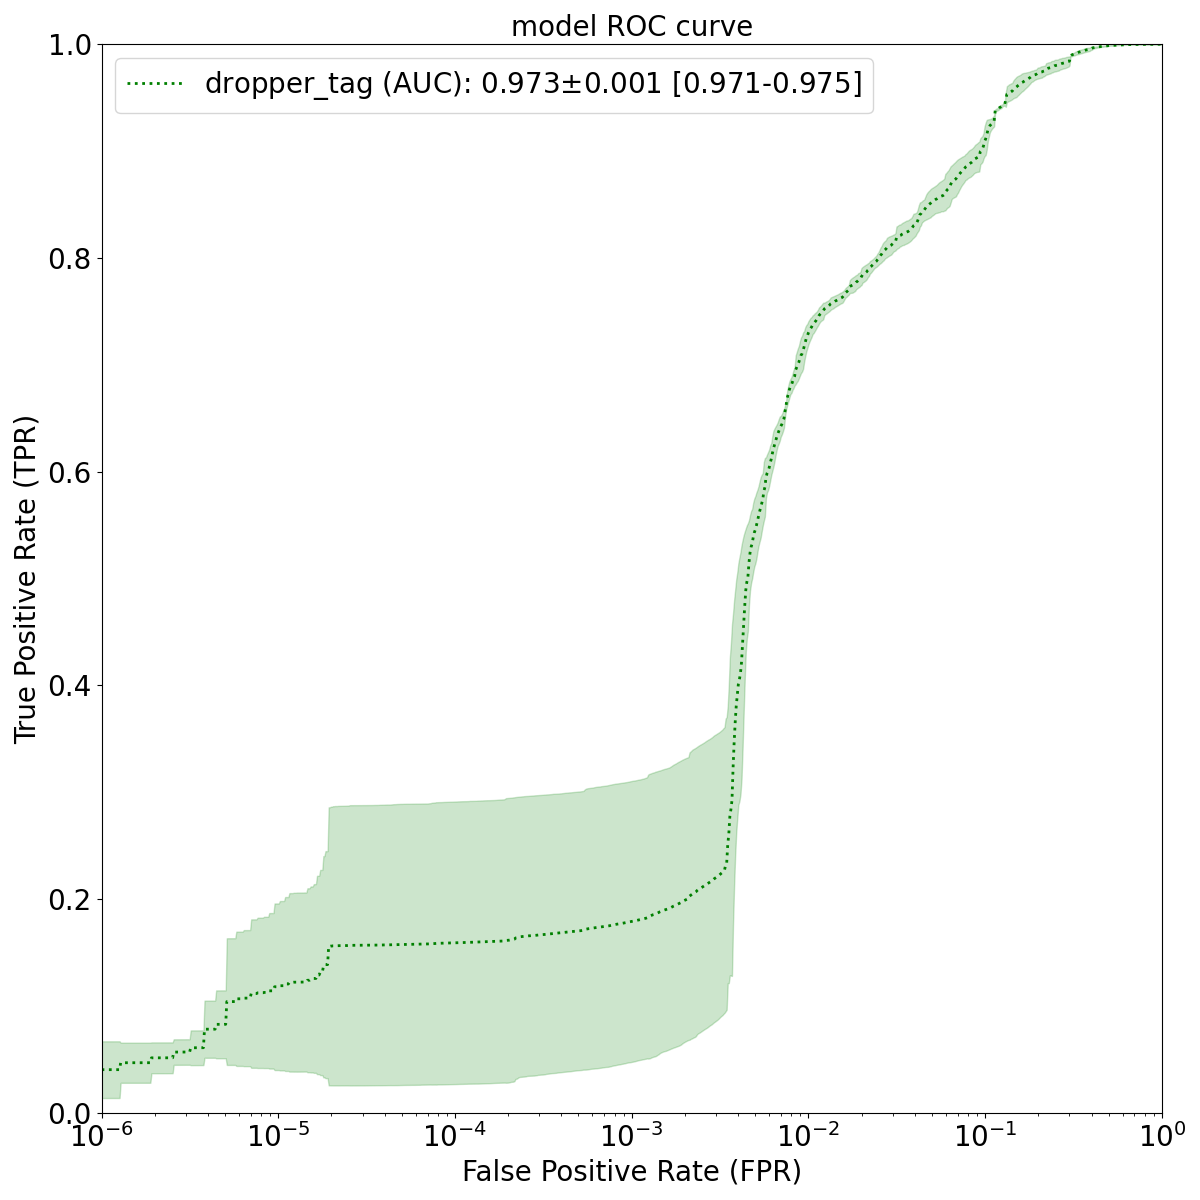
\includegraphics[width=0.6\textwidth]{./results/dropper_tag_roc_jointEmbedding.png}
        \vspace*{-0.2cm}
        \caption[Dropper Tag prediction task Joint Embedding ROC curve]{ROC curve and AUC statistics of \textBF{Joint Embedding} model for the \textbf{Dropper Tag}. The line represents the \textit{mean} TPR at a given FPR, while the shaded region represents the \textit{standard deviation}. Statistics were computed over \textBF{3} training runs, each with random parameter initialization.}
        \label{fig:dropperTagRocJointEmbedding}
    \end{figure}
}

\newcommand{\dropperTagRocProposedMethod}{
    \begin{figure}[H]
        \vspace*{-0.5cm}
        \centering
        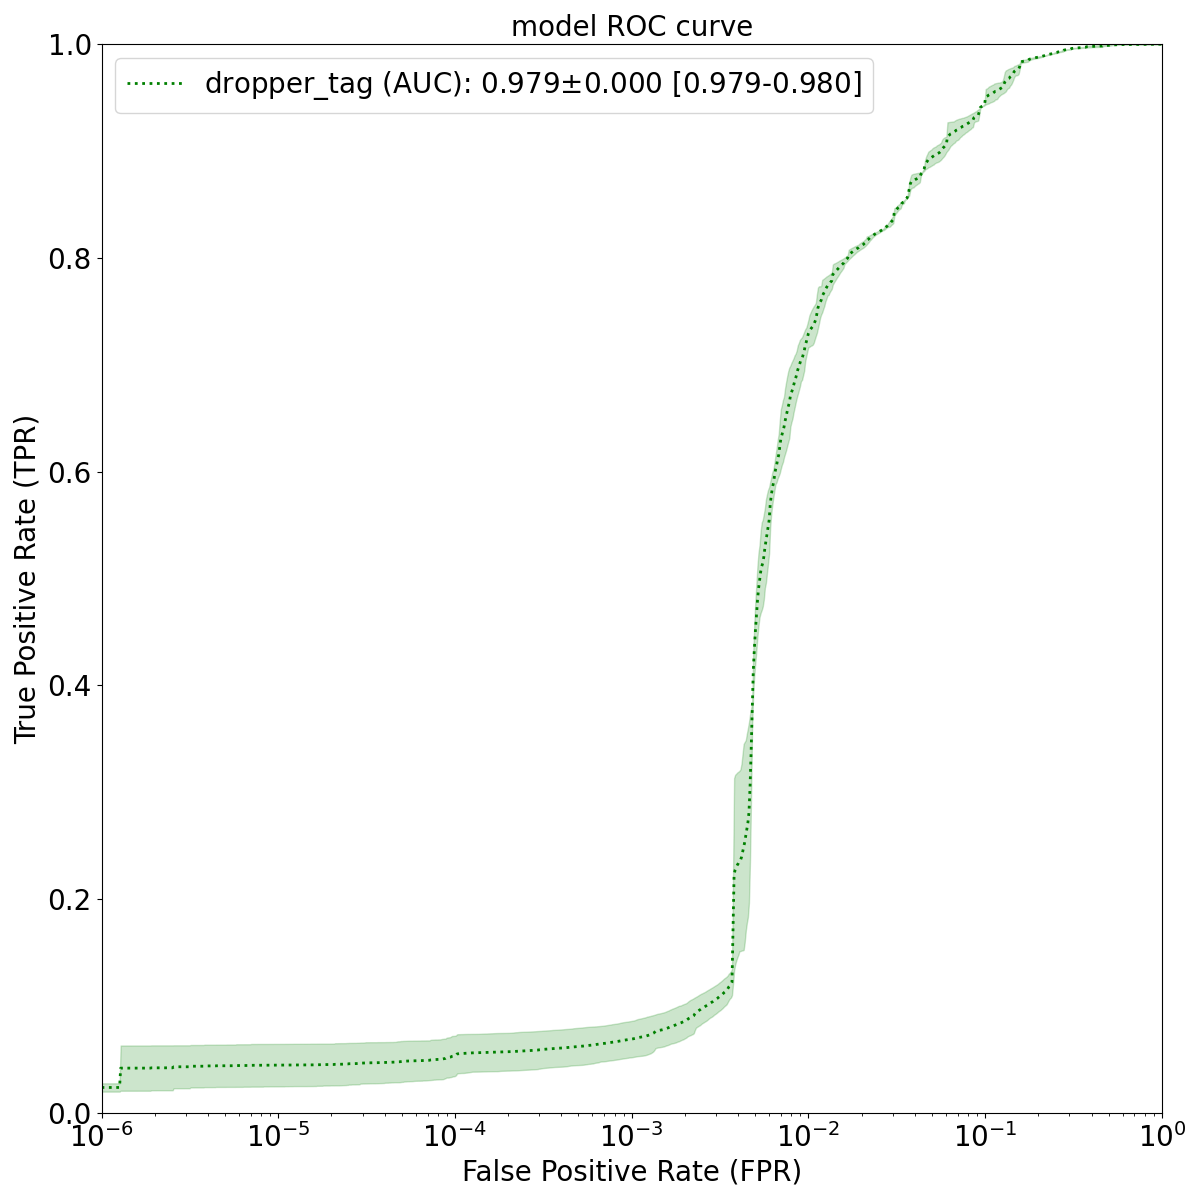
\includegraphics[width=0.6\textwidth]{./results/dropper_tag_roc_proposedModel.png}
        \vspace*{-0.2cm}
        \caption[Dropper Tag prediction task Proposed Model ROC curve]{ROC curve and AUC statistics of \textBF{Proposed Model} for the \textbf{Dropper Tag}. The line represents the \textit{mean} TPR at a given FPR, while the shaded region represents the \textit{standard deviation}. Statistics were computed over \textBF{3} training runs, each with random parameter initialization.}
        \label{fig:dropperTagRocProposedModel}
    \end{figure}
}
